\section{Introduction} \label{sec:intro}

%the necessity of having audit logging correctness (practical examples)
Audit logging is a prevalent mechanism used to capture the runtime events for the purpose of post-facto analysis, user accountability, diagnostics, security in-depth, etc. In this regard, enabling systems to generate necessary and sufficient logs plays a crucial role to meet the goals of audit logging. However, inadequate audit logging has been recognized as common problem in software development \cite{cwe778,owasp-top-ten}. While the audit log inadequacy  problem can be solved by naively recording massive volume of information at runtime, this approach incurs inefficiency in performance  and response to different security incidents \cite{cwe779}. For example, industrial control systems may suffer from the lack of monitoring audit logs in realtime to identify the security breaches \cite{controlsys}. Correctness of audit logging ensures to only record the necessary information. 

%what has been done previously for audit logging correctness
Information-algebraic \cite{Kohlas14}  models have been used within the last decade to provide semantic frameworks for audit logging. This has been accomplished by interpreting audit logs as well as the runtime structure of processes as information-algebraic elements, intuitively reflecting on their information content. Correct audit logging relies on this algebraic interpretation by comparing the information content of audit logs vs. the programs at runtime. Using this semantic framework, an implementation model has been proposed for linear processes that ensures correct audit logging, leveraging program instrumentation techniques \cite{post16}. The same framework has also been employed to identify and analyze direct information flows in Java-like settings \cite{amir-skalka-plas16, jcs20}. This semantic framework has also inspired the study of audit logging correctness in concurrent systems \cite{lsfa20}, which facilitates to log an event if one or more trigger events have occurred on the same or other concurrent components. The audit logging requirements can be specified with Horn clauses, where each event is a call to a function in a concurrent component, associated with its contextual information, e.g., the time of occurrence. 

%reason to focus on microservices(practicality)
Using microservices has become a popular approach in application development in recent years, and many organizations report success in its adoption \cite{Reilly}. Some surveys show more than $70\%$ of partial or full adoption worldwide in recent years \cite{Statista}. In this approach, a system is decomposed into multiple standalone loosely-coupled components, called microservices. Each microservice has its own database, and can run on a separate machine, VM, or container. Microservices commonly communicate with each other through RESTful APIs. The accommodated  modularity by a microservices-based system provides better maintainability which results in improved security, feature updates, and the ability to continue operating (at least partially)  despite the failure of one or more components. Microservices-based applications are architecturally concurrent and thus are good candidates to study the effectiveness of the aforementioned framework for audit logging in concurrent environments. 

%what does this paper aim at, the solution
Based on the implementation model for audit logging in concurrent systems \cite{lsfa20}, in a previous work \cite{stpsa21} we have described an instrumentation tool for Java microservices that are built on Spring framework. The tool supports audit logging requirements that can be specified by Horn clauses, according to which the instrumentation tool modifies different microservices so that concurrent audit logging is supported by the whole system. To accomplish this, the instrumented services may contact a Prolog engine to communicate the Horn clause specification of the logging requirements as well as the trigger and logging events. The Prolog engine is used to deduce whether logging in a certain microservice must take place. 

In this paper, we go beyond Horn clauses to specify audit logging requirements and study a sequel to the aforementioned instrumentation tool, where we can use a more expressive class of audit logging requirements to specify the conditions upon which logging must happen. The formal implementation model of correct audit logging in concurrent systems with the extended audit logging requirements is described elsewhere \cite{amirmoh-tr21}. Our proposed tool for Java microservices relies on this implementation model. Since audit logging requirements are extended beyond Horn clauses, our tool cannot simply communicate the logging requirements directly to a Prolog engine. We propose an algorithm through which Prolog is used to deduce intermediary candidate events to be logged and  filter out the ones that do not satisfy logging preconditions.

In the following, we describe an illustrative example that demonstrates the need to go beyond Horn clauses to specify audit logging requirements.

% an example
\textbf{\textit{Example: Microservices-based medical records system.}}
Let's consider a medical records system (MRS) with microservices architecture. Among numerous services of such system, this example assumes the existence of at least the following: 1) A front-end service that authenticates the users and multiplexes their queries to the back-end services,  2) an authorization system that controls access to system resources, and 3) a patient service that manages patient information. Figure \ref{fig:mrs-mics} demonstrates these microservices in a high-level manner. One common authorization-related operation in healthcare systems is to ``break-the-glass'' \cite{matthews-gaebel-hie09} in critical scenarios, which refers to accessing certain information (e.g., patient medical history) without any mediating authorization checks. After a user breaks the glass, actions of that user is recorded in the log for a posteriori analysis and establish user accountability.  A first attempt to specify the policy could be \emph{``Store in the log all accesses to patient medical history by a user who has already broken the glass''.}  This policy can be specified in Horn clause logic, and for which previous work proposes an implementation model \cite{lsfa20} and a tool for Java-based  microservices \cite{stpsa21}.  

\begin{figure} 
	\centering
	\fbox{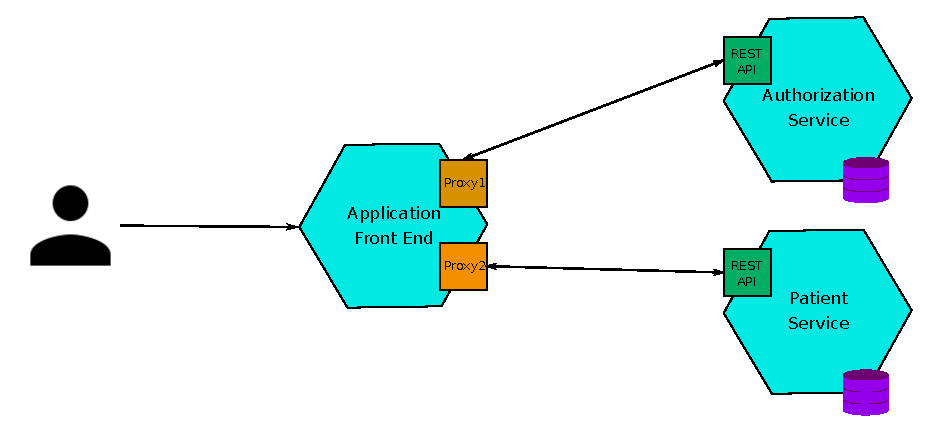
\includegraphics[width=0.45\textwidth]{./figs/mrs-mics2.eps}}
	\caption{An Example MRS.}
	\label{fig:mrs-mics}
\end{figure}

However, the aforementioned policy entails to log all such accesses indefinitely. In reality, breaking the glass is deactivated once the critical situation is resolved. Therefore, we may consider some dual capability ``mend-the-glass'' that restores access control and enforces it fully, if the glass is already broken. Having this capability, the example break-the-glass policy can be restated as follows: \emph{``Store in the log all accesses to patient medical history by a user who has already broken the glass and has not mended it afterwards''.}  This updated more realistic specification goes beyond Horn clauses in expressivity.

Therefore, a compelling next step is to consider a more powerful instrumentation tool to implement logging specifications that support extended preconditions like the one discussed above. Our instrumentation tool relies on models of correct audit logging which support more expressive classes of logging specifications.



%paper outline

\textbf{\textit{Paper outline.}}
The rest of the paper is organized as follows. In Section \ref{sec:implmodel}, we review the formal implementation model, discussing an instrumentation algorithm for systems in $\pi$-calculus. In Section \ref{sec:impl}, we discuss our tool to instrument microservices in Java Spring. In addition, we present a demo of a microservices-based MRS, and its instrumentation by our tool. 
%Section \ref{sec:eval} provides an empirical analysis of the instrumented applications, focusing on runtime overhead. 
%In Section \ref{sec:discussion}, we describe the limitations of this work, and potential future work. 
%Related work is discussed in Section \ref{sec:relwork}. Finally, Section \ref{sec:conclusion} concludes the paper.
Section \ref{sec:rwc} disucsses the related work and concludes the paper.